%!TEX TS-program = xelatex
%!TEX encoding = UTF-8 Unicode

\documentclass[tikz]{standalone}
\usetikzlibrary{math}

\begin{document}
  % borrow the code from http://latex-community.org/know-how/513-tikz-math
  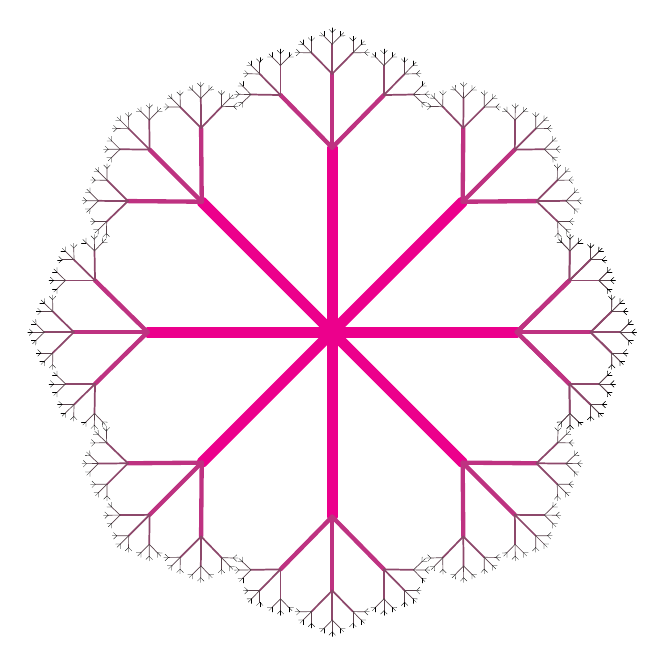
\begin{tikzpicture}[scale=.06pt]
    \tikzmath{
      % --------------------------
      % the parameters of the tree
      % --------------------------
      \power=2.5; % the scale base factor
      \deviation=44.5; % the angle between the 3 child edges
      \numsteps=5; % number of levels
      let \startcolor=magenta; % the start color
      let \endcolor=black; % the end color
      % -------------------------------------------------------------------------
      % the function that draw one edge and call itself to draw the 3 child edges
      % -------------------------------------------------------------------------
      function Branch(\x,\y,\rotate,\step){
        \step=\step-1; % stops drawing if step < 0
        if (\step >= 0) then {
          \mix = int(100*\step/(\numsteps-1)); % the color mix parameter is in [0,100]
          \scale = \power^\step; % the scale factor
          { % "print" the tikz command that draw the edge
            \draw[shift={(\x pt,\y pt)}, rotate=\rotate, scale=\scale,
                  color=\startcolor!\mix!\endcolor, line width=\scale*.1 pt,
                  line cap=round]
              (0,0)--(1,0) coordinate(newbase);
          };
          coordinate \b; \b1 = (newbase); % the new base point
          for \a in {-\deviation,0,\deviation}{
            Branch(\bx1,\by1,mod(\rotate+\a,360),\step); % draw one child edge
          };
        };
      };
      % ----------------------
      % draw the four branches
      % ----------------------
      for \angle in {0,45,...,360}{
        Branch(0,0,\angle,\numsteps);
      };
    }
  \end{tikzpicture}
\end{document}
